\section{System Architecture}
This section presents an overview of the platform's system architecture, which is designed to be modular, scalable, and responsive for data annotation workflows. Figure~\ref{fig:system-architecture} illustrates the interconnected components that form the platform's ecosystem, comprising a client-side web application, a cloud-hosted serverless backend, and integrations with specialized external services.

\begin{figure}[ht]
\centering
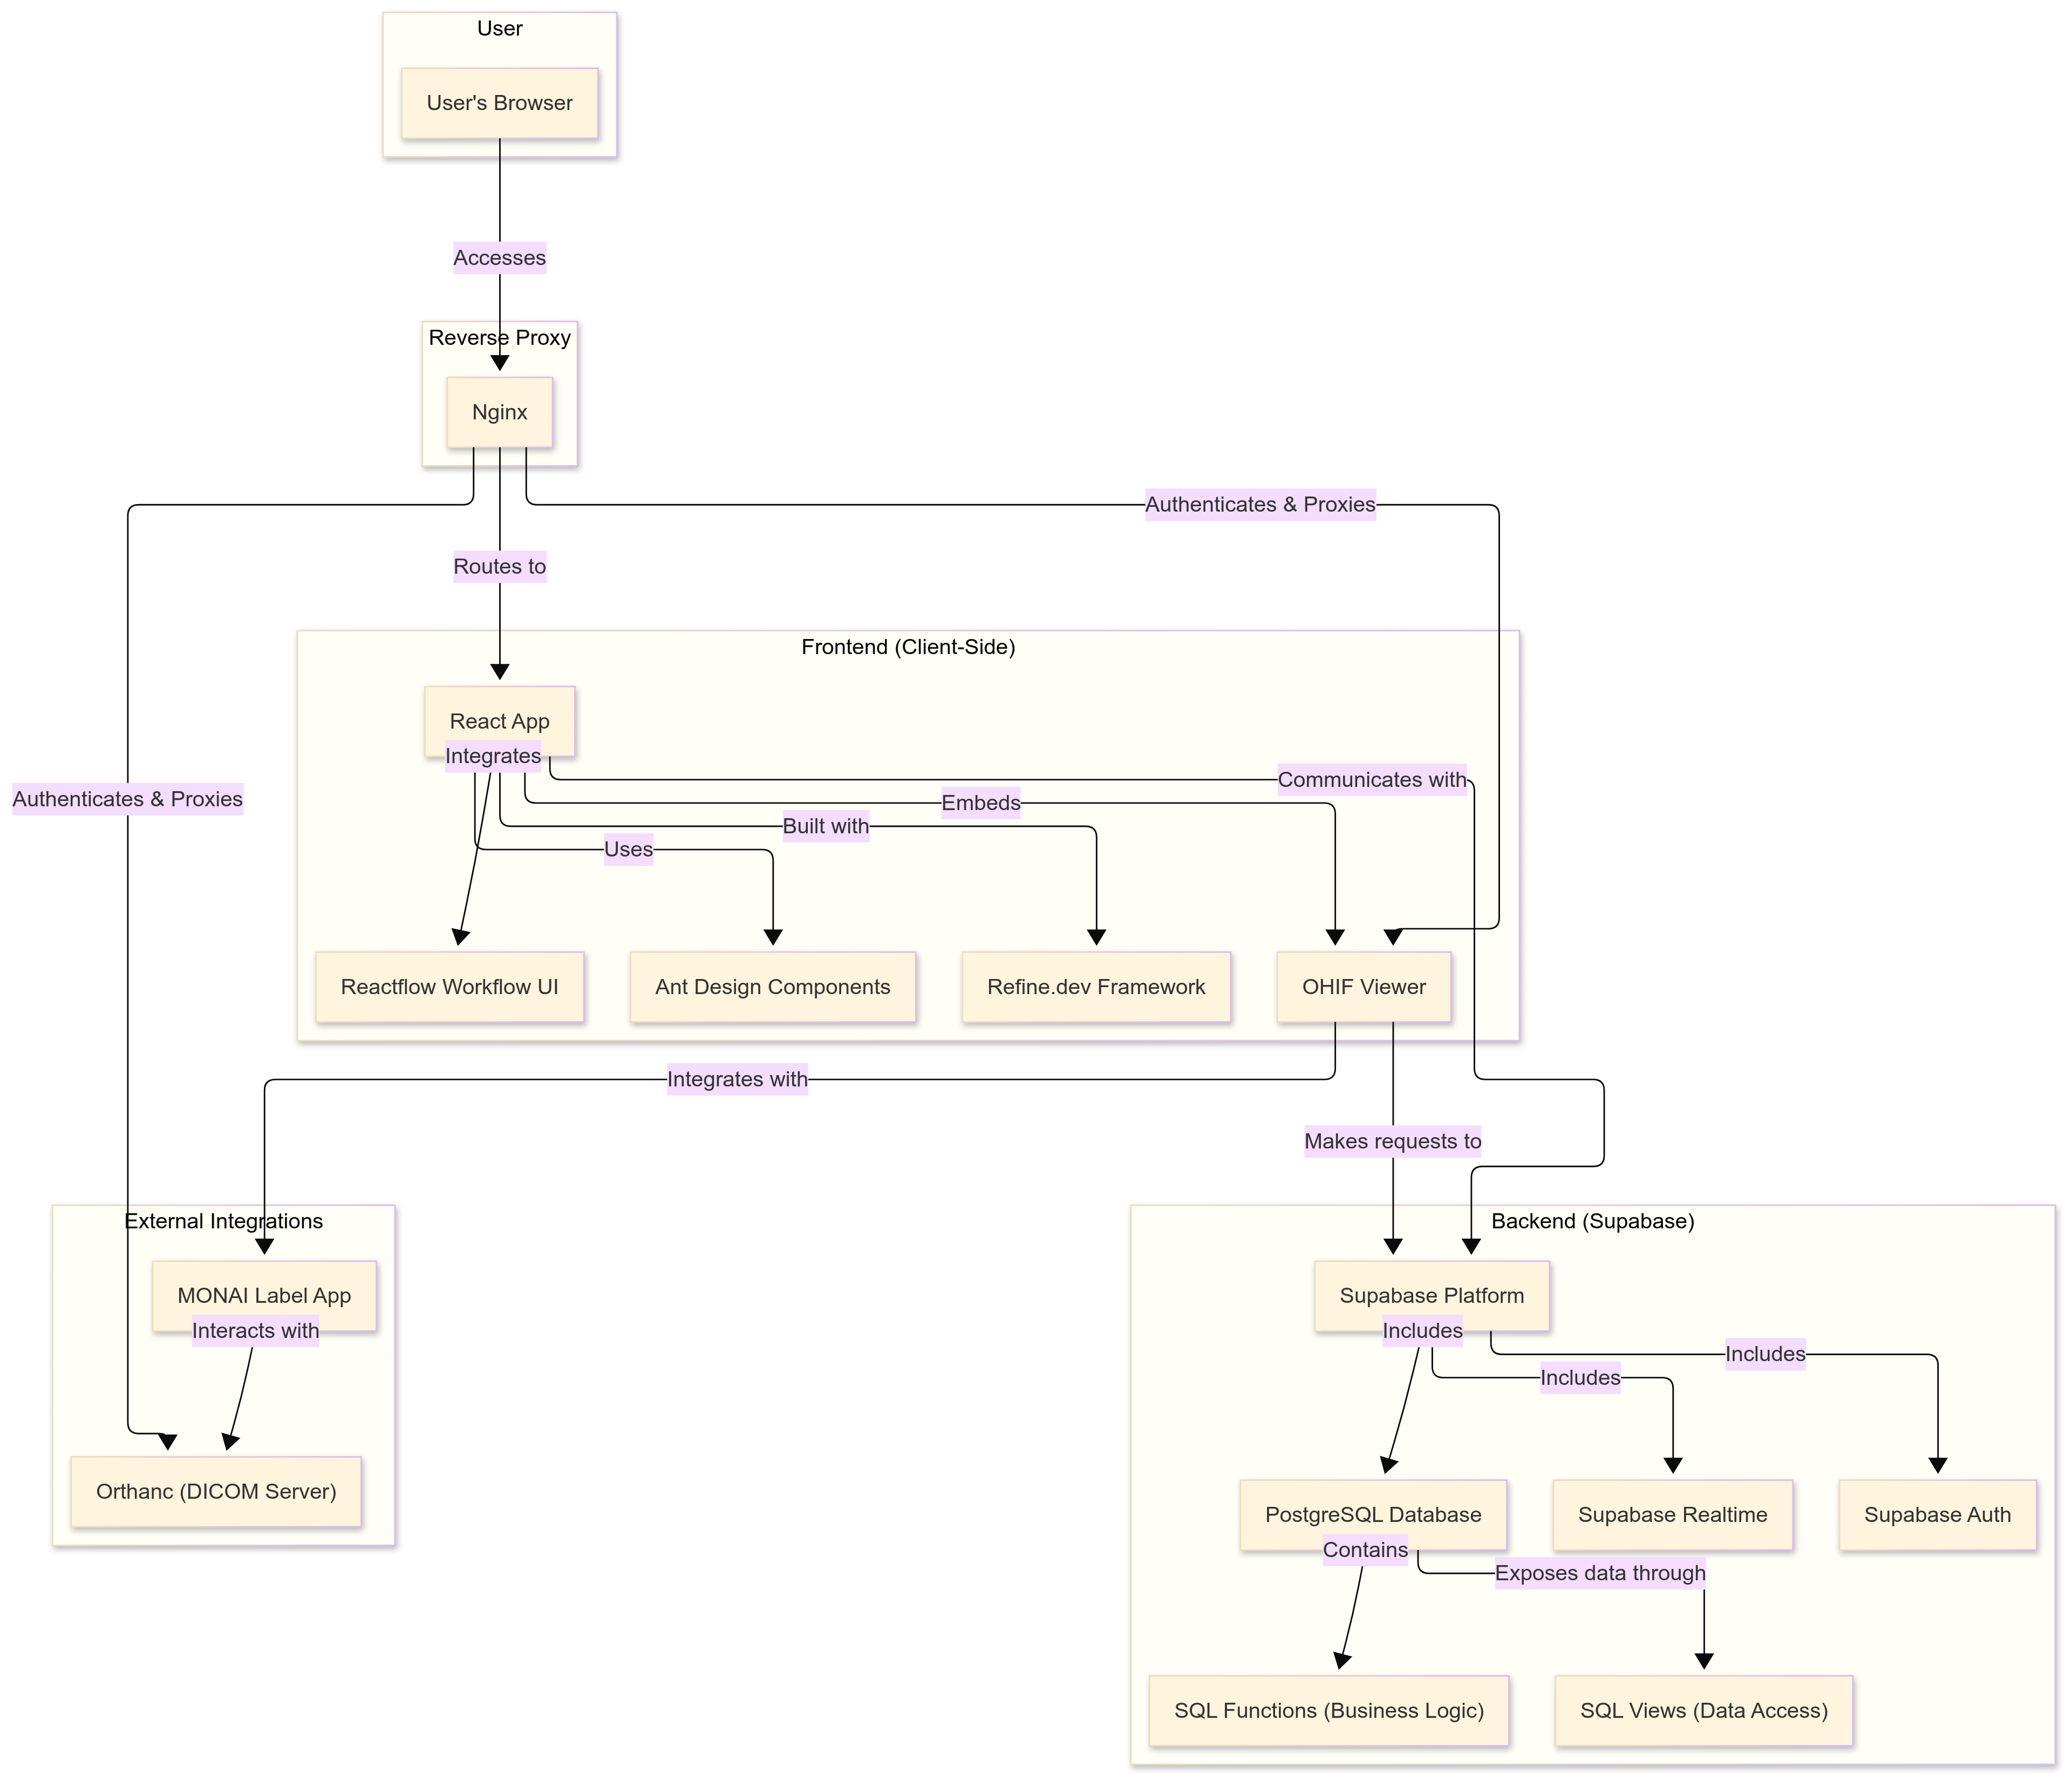
\includegraphics[width=0.9\textwidth]{content/resources/architecture.png} % Placeholder for diagram
\caption{Overall System Architecture.}
\label{fig:system-architecture}
\end{figure}

\subsection{Client-Side Application}
The client-side application provides the user interface for interacting with the platform. It runs within a standard web browser and is responsible for data presentation, user input, and real-time visualization of workflows and annotations.

\subsubsection{Web Browser Interface}
Users access the platform through a modern web browser. A dedicated Nginx reverse proxy manages traffic routing, serving the frontend assets and securely proxying specific requests to external services where necessary.

\subsubsection{Frontend Technologies}
The user interface is built as a React application, utilizing the \texttt{Refine.dev} framework to streamline development of CRUD operations and application logic. Visual consistency is provided by \texttt{Ant Design} components. For workflow design, the platform integrates \texttt{XYFlow} to enable interactive graphical editing of workflow graphs. Additionally, the \texttt{OHIF Viewer} is embedded for specialized medical imaging annotation and viewing functionalities.

\subsection{Backend Services (Supabase)}
The backend operates on a serverless architecture, leveraging Supabase to provide core database, authentication, and real-time capabilities.

\subsubsection{Supabase Ecosystem}
The entire backend resides within the Supabase platform, which provides a comprehensive suite of cloud-hosted services. This includes a robust \texttt{PostgreSQL Database} for all data storage, \texttt{Supabase Auth} for user authentication and authorization, and \texttt{Supabase Realtime} for instant data synchronization to connected clients.

\subsubsection{Data Storage and Logic}
All persistent data and core business logic are managed within the PostgreSQL database. This includes structured data for projects, tasks, and users, along with JSONB fields for flexible workflow stage configurations. Complex operations and state transitions are encapsulated within \texttt{SQL Functions}, which serve as the primary executable logic, while \texttt{SQL Views} provide abstracted and secure data access layers for the frontend.

\subsection{External Integrations}
The platform extends its capabilities through seamless integration with specialized external systems, particularly relevant for advanced medical imaging and AI-assisted annotation.

\subsubsection{Specialized Tools}
For AI-assisted medical image labeling, the platform integrates with the \texttt{MONAI Label App}, a server-side framework that offers machine learning model inference. Additionally, \texttt{Orthanc}, a lightweight DICOM server, functions as a primary source for medical image data, providing seamless access to studies for annotation tasks.